%%%%%%%%%%%%%%%%%%%%%%%%%%%%%%%%%%%%%%%%%
% Template
% LaTeX Template
% Version 1.0 (December 8 2014)
%
% This template has been downloaded from:
% http://www.LaTeXTemplates.com
%
% Original author:
% Brandon Fryslie
% With extensive modifications by:
% Vel (vel@latextemplates.com)
%
% License:
% CC BY-NC-SA 3.0 (http://creativecommons.org/licenses/by-nc-sa/3.0/)
%
% Authors:
% Sabbir Ahmed, Jeffrey Osazuwa, Howard To, Brian Weber
% 
%%%%%%%%%%%%%%%%%%%%%%%%%%%%%%%%%%%%%%%%%

\documentclass[paper=usletter, fontsize=12pt]{article}
%%%%%%%%%%%%%%%%%%%%%%%%%%%%%%%%%%%%%%%%%
% Contract Structural Definitions File Version 1.0 (December 8 2014)
%
% Created by: Vel (vel@latextemplates.com)
% 
% This file has been downloaded from: http://www.LaTeXTemplates.com
%
% License: CC BY-NC-SA 3.0 (http://creativecommons.org/licenses/by-nc-sa/3.0/)
%
%%%%%%%%%%%%%%%%%%%%%%%%%%%%%%%%%%%%%%%%%

\usepackage{geometry} % Required to modify the page layout
\usepackage{multicol}
\usepackage{amsmath}
\usepackage{amssymb}

\usepackage[pdftex]{graphicx}
\usepackage{wrapfig}
\usepackage[font=scriptsize, labelfont=bf]{caption}
\usepackage[utf8]{inputenc} % Required for including letters with accents
\usepackage[T1]{fontenc} % Use 8-bit encoding that has 256 glyphs

\usepackage{avant} % Use the Avantgarde font for headings
\usepackage{courier}
\usepackage{xparse}
\usepackage{xcolor}
\usepackage{listings}  % for code verbatim and console outputs

\setlength{\textwidth}{16cm} % Width of the text on the page
\setlength{\textheight}{23cm} % Height of the text on the page
\setlength{\oddsidemargin}{0cm} % Width of the margin - negative to move text left, positive to move it right
\setlength{\topmargin}{-1.25cm} % Reduce the top margin

\setlength{\parindent}{0mm} % Don't indent paragraphs
\setlength{\parskip}{2.5mm} % Whitespace between paragraphs
\renewcommand{\baselinestretch}{1.5}

\definecolor{green}{rgb}{0.18, 0.55, 0.34}

\graphicspath{ {figures/} }
\captionsetup[table]{skip=10pt}

\lstset{language=C, keywordstyle={\bfseries \color{black}}}

% defines algorithm counter for chapter-level
\newcounter{nalg}[section]

%defines appearance of the algorithm counter
\renewcommand{\thenalg}{\thesection .\arabic{nalg}}

% defines a new caption label as Algorithm x.y
\DeclareCaptionLabelFormat{algocaption}{Algorithm \thenalg}

% defines the algorithm listing environment
\lstnewenvironment{pseudocode}[1][] {
    \refstepcounter{nalg}  % increments algorithm number
    \captionsetup{font=normalsize, labelformat=algocaption, labelsep=colon}
    \lstset{
        breaklines=true,
        mathescape=true,
        numbers=left,
        numberstyle=\scriptsize,
        basicstyle=\footnotesize\ttfamily,
        keywordstyle=\color{black}\bfseries,
        keywords={input, output, return, parallel, function, for, to, in, if,
        else, foreach, while, and, or, new, print},
        xleftmargin=.04\textwidth,
        #1
    }
}{}

\renewcommand{\familydefault}{\sfdefault}  % default font for entire document
 % specifies the document layout and style

%----------------------------------------------------------------------------------------

% document info command
\newcommand{\documentinfo}[5]{
    \begin{centering}
        \parbox{2in}{
        \begin{spacing}{1}
            \begin{flushleft}
                \begin{tabular}{l l}
                    #1 \\
                    #2 \\
                    #3 \\
                \end{tabular}\\
                \rule{\textwidth}{1pt}
            \end{flushleft}
        \end{spacing}
        }
    \end{centering}
}

\begin{document}


    \documentinfo{Midterm 1: Extra Credit Code Snippet}{Sabbir Ahmed}{Date: \today}
    \vspace{-0.1in}

    \section{Usefulness of \texttt{`printf()`}}
    \inlsnip{printf()} is one of the most useful functions for beginners in the C programming language. It is a very helpful tool when it comes to debugging, checking statuses of dynamic variables, or simply printing to console. What many users are unaware of is that the function may be used for other very useful tricks.

    The formal declaration of the function is:

\begin{lstlisting}
    int printf(const char *format, ...)
\end{lstlisting}

    where the returning type \inlsnip{int} is in fact the total number of characters written. A negative number is returned on failure. This property can be used in interesting ways, such as described in the snippet below: \\

\begin{lstlisting}
    #include <stdio.h>

    int main() {

        char hello_world[] = "hello world";

        printf("%d\n", printf(hello_world));
        return 0;

    }
\end{lstlisting}

    The snipper described will build with a warning:

    \begin{figure}[ht]
        \begin{center}
            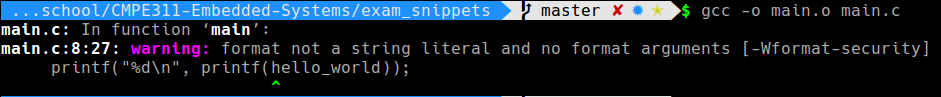
\includegraphics[width=1\textwidth]{build1.png}
            \caption{Building Snippet 1} \label{fig:build1}
        \end{center}
    \end{figure}

    And when ran, will output interesting results:

    \begin{figure}[ht]
        \begin{center}
            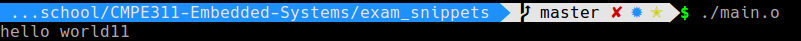
\includegraphics[width=1\textwidth]{run1.png}
            \caption{Running Snippet 1} \label{fig:run1}
        \end{center}
    \end{figure}

    The output on the console consisted of the inner \inlsnip{printf()} function printing out the string first, then returning its number of characters to be dumped by the outer \inlsnip{printf()}.

    The function can also be used for a very simple debugging purpose - finding the data type of a variable. If possible, \inlsnip{printf()} will attempt to output any valid arguments passed to it with its corresponding formatting string. However, passing in an incompatible data type variable with the "\%d" string formatter will result in most compilers warning the user during the build. The warning will include the actual data type of the variable, such as the following snippet:

\begin{lstlisting}
    #include <stdio.h>

    int main() {

        char hello_world[] = "hello world";

        printf("%d\n", hello_world);
        return 0;

    }
\end{lstlisting}

    The snippet will invoke the following warning when built:

    \begin{figure}[ht]
        \begin{center}
            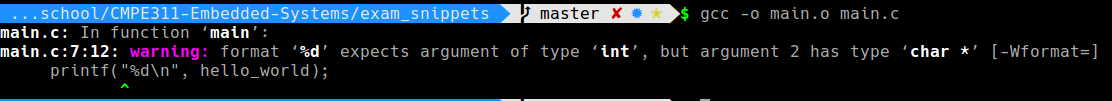
\includegraphics[width=1\textwidth]{build2.png}
            \caption{Building Snippet 2} \label{fig:build2}
        \end{center}
    \end{figure}

    thus, notifying the user of their variable's data type. Of course, printing out the variable with the wrong string formatter would not be very useful!

    \begin{figure}[ht]
        \begin{center}
            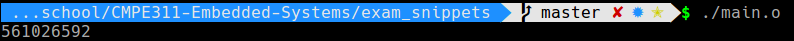
\includegraphics[width=1\textwidth]{run2.png}
            \caption{Running Snippet 2} \label{fig:run2}
        \end{center}
    \end{figure}

\end{document}
